\newpage
\section{Projekt i~implementacja systemu}

\subsection{Idea systemu i~przypadki użycia}

System \texttt{dex-arb-analyzer} jest narzędziem analitycznym dla jednego aktora, badacza rynku.
Realizuje jeden zasadniczy przepływ. Dla wybranej pary tokenów i~okna czasowego pobiera z~węzła
Ethereum historię obu puli (Uniswap~V2 i~Sushiswap), odtwarza ich stan po każdym bloku, wykrywa
bloki z~rozbieżnością cenową powyżej progu i~ocenia każdą taką okazję czterema modelami.
Następnie sprawdza w~historii łańcucha, czy okazja została faktycznie skonsumowana. Uzyskane
etykiety służą do kalibracji i~uczenia modeli oraz do ich porównania. Przypadki użycia
(rys.~\ref{fig:uc}) obejmują:
\begin{itemize}[nosep]
  \item zlecenie pobrania danych dla puli i~okna (\emph{ingest}) oraz śledzenie postępu zadania,
  \item zlecenie analizy pary w~oknie (stany bloków, okazje, oceny modeli),
  \item zlecenie weryfikacji retrospektywnej okazji,
  \item przegląd szeregów czasowych (ceny, rozbieżność, gaz, oceny) i~listy okazji z~podglądem
        szczegółów pojedynczej okazji, w~tym aktywacji reguł rozmytych,
  \item kalibrację heurystyki (baseline~v2) i~trening ANFIS na wybranych oknach,
  \item porównanie modeli (macierze pomyłek, krzywe ROC, histogramy ocen),
  \item obserwację bieżącego stanu puli w~trybie ,,na żywo''.
\end{itemize}
\begin{figure}[H]\centering% Diagram przypadków użycia
\begin{tikzpicture}[dg]
\node[actor] (badacz) at (0,1.0) {Badacz};
\node[actor] (worker) at (0,-6.3) {Proces\\\texttt{worker}};
\node[actor] (rpc) at (13.2,-1.9) {Węzeł RPC};

\foreach \i/\t in {1/{Zleć pobranie danych (pula, okno)}, 2/{Zleć analizę pary w~oknie},
                   3/{Zleć weryfikację okazji}, 4/{Przeglądaj szeregi i~okazje},
                   5/{Kalibruj / trenuj model}, 6/{Porównaj modele}, 7/{Obserwuj stan na żywo}}
  \node[uc] (u\i) at (6.6, 2.9-1.15*\i) {\t};
\node[uc] (u8) at (6.6,-6.3) {Wykonaj zadanie z~kolejki};

\node[draw=dgLine, rounded corners=5pt, fit=(u1)(u8), inner sep=9pt] (box) {};
\node[anchor=south west, font=\footnotesize\ttfamily, text=dgLine] at ([yshift=1pt]box.north west) {dex-arb-analyzer};

\foreach \i in {1,...,7} \draw[dep, draw=dgLine] (badacz.east) -- (u\i.west);
\draw[dep, draw=dgLine] (worker.east) -- (u8.west);
\draw[ctl] (u8.north) -- node[lbl, right, xshift=2pt] {\textit{<<include>>} ingest, analiza, weryfikacja, trening} (u7.south);
\foreach \i in {1,3,7} \draw[dep, draw=dgLine] (rpc.west) -- (u\i.east);
\end{tikzpicture}

\caption{Diagram przypadków użycia systemu (opracowanie własne)}\label{fig:uc}\end{figure}

\subsection{Architektura}

System jest monorepozytorium npm (TypeScript, Node~$\geq$~20) złożonym z~ośmiu pakietów
o~rozłącznych odpowiedzialnościach (rys.~\ref{fig:arch}). Pakiet \texttt{core} zawiera arytmetykę
AMM, cechy, modele oceny i~metryki ewaluacji; jest to czysty kod bez dostępu do bazy i~sieci,
w~całości testowalny jednostkowo. Pakiet \texttt{db} definiuje schemat PostgreSQL (Drizzle ORM)
i~migracje, a~\texttt{shared} kontrakty danych (schematy zod) wspólne dla API i~interfejsu.
Za pobieranie zdarzeń i~bloków z~węzła RPC odpowiada \texttt{ingest}. Pakiet \texttt{analysis}
odtwarza stany, wykrywa okazje, ocenia je modelami, prowadzi weryfikację retrospektywną
i~buduje zbiór uczący. Zadania z~kolejki wykonuje \texttt{worker}, serwer HTTP (Fastify) to
\texttt{api}, a~interfejs użytkownika (React, Vite, TanStack Query, Recharts) to \texttt{web}.

Przepływ danych jest jednokierunkowy: RPC $\rightarrow$ \texttt{ingest} $\rightarrow$ baza
$\rightarrow$ \texttt{analysis} $\rightarrow$ baza $\rightarrow$ \texttt{api} $\rightarrow$
\texttt{web}. Zadania długotrwałe (pobieranie, analiza, weryfikacja, trening) nie są wykonywane
w~procesie API. Trafiają jako wiersze do tabeli \texttt{jobs} i~podejmuje je osobny proces
\texttt{worker}, więc interfejs pozostaje responsywny, a~zadania można wznowić po awarii. Każdy
krok jest idempotentny: ponowne uruchomienie nie duplikuje danych (wstawianie
z~\texttt{ON CONFLICT}, klucze naturalne).
\begin{figure}[H]\centering\resizebox{\linewidth}{!}{% Diagram komponentów i przepływu danych
\begin{tikzpicture}[dg, x=1cm, y=1cm,
  pkg/.append style={minimum width=28mm, minimum height=12mm},
  lib/.append style={minimum width=28mm, minimum height=12mm},
  ext/.append style={minimum width=28mm, minimum height=12mm}]
% rząd A: przepływ danych
\node[ext] (rpc)    at (0,0)  {Węzeł RPC\\(archiwalny)};
\node[pkg] (ingest) at (4,0)  {\texttt{ingest}};
\node[ext] (db)     at (8,0)  {PostgreSQL\\(dane, kolejka \texttt{jobs})};
\node[pkg] (api)    at (12,0) {\texttt{api}\\(Fastify)};
\node[pkg] (web)    at (16,0) {\texttt{web}\\(React)};
% rząd B
\node[pkg] (analysis) at (8,-3)  {\texttt{analysis}};
\node[lib] (core)     at (12,-3) {\texttt{core}\\(AMM, cechy, modele)};
\node[lib] (shared)   at (16,-3) {\texttt{shared}\\(DTO zod)};
% rząd C
\node[pkg] (worker) at (8,-6) {\texttt{worker}\\(wykonuje zadania)};

\draw[flow] (rpc) -- node[lbl,above] {logi, bloki} (ingest);
\draw[flow] (ingest) -- node[lbl,above] {zdarzenia} (db);
\draw[flow] (db) -- node[lbl,above] {SQL} (api);
\draw[flow] (api) -- node[lbl,above] {JSON} (web);
\draw[flow,<->] (db) -- node[lbl,right] {stany, okazje, oceny} (analysis);
\draw[flow] (rpc.south) |- node[lbl,pos=.75,above] {paragony transakcji} (analysis.west);
\draw[ctl] (worker) -- node[lbl,right] {uruchamia} (analysis);
\draw[ctl] (worker.west) -- ++(-4.6,0) |- node[lbl,pos=.22,right] {uruchamia} (ingest.west);
\draw[dep] (core) -- (analysis);
\draw[dep] (core) -- (api);
\draw[dep] (shared) -- (web);
\draw[dep] (shared) -- (core);

\node[font=\scriptsize, text=dgLine, anchor=west] at (-1.6,-7.4) {
  \tikz\draw[flow] (0,0)--(.5,0); przepływ danych\qquad
  \tikz\draw[ctl] (0,0)--(.5,0); sterowanie\qquad
  \tikz\draw[dep] (0,0)--(.5,0); zależność kodu};
\end{tikzpicture}
}
\caption{Architektura systemu: pakiety i~przepływ danych (opracowanie własne)}\label{fig:arch}\end{figure}

\subsection{Model danych}

Schemat bazy (rys.~\ref{fig:erd}) ma trzy warstwy. Warstwa konfiguracji to \texttt{dexes}
(giełdy z~adresem fabryki i~prowizją), \texttt{tokens}, \texttt{pairs} (para logiczna z~tokenem
bazowym i~kwotowanym), \texttt{pools} (pula danej giełdy dla pary; unikalna kombinacja
\texttt{(dex\_id, pair\_id)}) oraz \texttt{windows} (okno analizy z~zakresem czasu i~bloków).
Dane surowe przechowują tabele \texttt{blocks} (znacznik czasu, \texttt{base\_fee}, mediana ceny
gazu w~wei), \texttt{sync\_events} i~\texttt{swap\_events} z~kluczem naturalnym
\texttt{(pool\_id, block, log\_index)} oraz \texttt{ingest\_ranges}, czyli rejestr pobranych
zakresów bloków ze statusem, który zapewnia wznawialność. Dane pochodne to \texttt{block\_states}
(stan pary w~każdym bloku okna: ceny obu puli, rozbieżność, TVL, cechy $S,G,L,M$, optymalna
transakcja, zysk brutto; klucz \texttt{(pair\_id, block)}), \texttt{opportunities} (bloki
z~rozbieżnością powyżej progu), \texttt{opportunity\_verifications} (status, transakcja
konsumująca, zysk zrealizowany, koszt gazu, trasa, etykieta), \texttt{scoring\_models} (model
z~parametrami w~JSON, oknami treningowymi i~metrykami) i~\texttt{model\_scores} (ocena każdego
modelu dla każdego bloku). Kolejkę zadań reprezentuje tabela \texttt{jobs}.

Rezerwy i~kwoty tokenów są przechowywane jako \texttt{numeric(40,0)} i~przetwarzane
w~TypeScript jako \texttt{bigint}, żeby arytmetyka kontraktu była odtworzona dokładnie.
Wielkości w~USD i~cechy mają typ \texttt{double precision}. Poprawność danych wymuszają
ograniczenia \texttt{CHECK} (dwanaście w~migracji \texttt{0007}): zakresy cech ($S\in[0,3]$,
$G\in[0,2]$, $L\in[0,100]$, $M\in[0,100]$), zakres oceny modelu $[0,100]$,
$\texttt{blocks\_to\_consumption}\in[0,3]$ oraz równoważność ,,istnieje transakcja konsumująca''
$\Leftrightarrow$ ,,status jest konsumpcją''. Migracje są jednokierunkowe. Baza jest w~całości
odtwarzalna z~RPC, więc cofnięcie schematu oznacza odtworzenie bazy od zera.
\begin{figure}[H]\centering\resizebox{\linewidth}{!}{% Schemat bazy danych (uproszczony ERD). PK podkreślone, FK kursywą.
\begin{tikzpicture}[dg, x=1cm, y=1cm,
  ent/.style={draw=dgLine, rectangle split, rectangle split parts=2, rectangle split part fill={dgHead,white},
              align=left, inner sep=3pt, text width=33mm, font=\scriptsize, rounded corners=1pt},
  rel/.style={->, draw=dgLine, line width=.5pt}]
% kolumna 1: konfiguracja / pochodne
\node[ent] (dexes)  at (0,4.6)  {\textbf{dexes}\nodepart{second}\underline{id}\\name, factory, fee\_bps};
\node[ent] (tokens) at (0,2.7)  {\textbf{tokens}\nodepart{second}\underline{address}\\symbol, decimals};
\node[ent] (pairs)  at (0,0.6)  {\textbf{pairs}\nodepart{second}\underline{id}\\symbol\\\textit{token\_base}, \textit{token\_quote}};
\node[ent] (bs)     at (0,-2.5) {\textbf{block\_states}\nodepart{second}\underline{\textit{pair\_id}, block}\\\textit{window\_id}, price\_a, price\_b\\spread\_pct, tvl\_min\_usd\\s, g, l, m, opt\_trade\_usd\\gross\_profit\_usd, direction};
\node[ent] (models) at (0,-6.1) {\textbf{scoring\_models}\nodepart{second}\underline{id}\\name, kind, version\\params, metrics (jsonb)\\trained\_on\_window\_ids};
% kolumna 2
\node[ent] (pools)   at (4.6,2.7)  {\textbf{pools}\nodepart{second}\underline{id}\\\textit{dex\_id}, \textit{pair\_id}\\address, token0, token1};
\node[ent] (windows) at (4.6,0.3)  {\textbf{windows}\nodepart{second}\underline{id}\\name, from\_ts, to\_ts\\from\_block, to\_block};
\node[ent] (opp)     at (4.6,-2.5) {\textbf{opportunities}\nodepart{second}\underline{id}\\\textit{pair\_id}, \textit{window\_id}, block\\spread\_pct, direction\\est\_profit\_usd};
\node[ent] (ver)     at (4.6,-6.1) {\textbf{opportunity\_verifications}\nodepart{second}\underline{\textit{opportunity\_id}}\\status, route\\consumer\_tx\_hash\\realized\_profit\_usd, gas\_cost\_usd\\blocks\_to\_consumption\\profitable\_consumed};
% kolumna 3: surowe / oceny / kolejka
\node[ent] (blocks) at (9.2,4.6)  {\textbf{blocks}\nodepart{second}\underline{number}\\timestamp, base\_fee\\gas\_price\_median, tx\_count};
\node[ent] (sync)   at (9.2,2.5)  {\textbf{sync\_events}\nodepart{second}\underline{\textit{pool\_id}, block, log\_index}\\tx\_hash, reserve0, reserve1};
\node[ent] (swap)   at (9.2,0.3)  {\textbf{swap\_events}\nodepart{second}\underline{\textit{pool\_id}, block, log\_index}\\tx\_hash, sender, to\\amount0/1\_in/out, gas\_price};
\node[ent, text width=38mm] (ranges) at (9.2,-2.0) {\textbf{ingest\_ranges}\nodepart{second}\underline{\textit{pool\_id}, from\_block, to\_block}\\status, error};
\node[ent, text width=39mm] (scores) at (9.2,-4.2) {\textbf{model\_scores}\nodepart{second}\underline{\textit{model\_id}, \textit{pair\_id}, block}\\score, label};
\node[ent] (jobs)   at (9.2,-6.5) {\textbf{jobs}\nodepart{second}\underline{id}\\type, params (jsonb), status\\progress, log, error, attempts};

\draw[rel] (pools.north) |- (dexes.east);
\draw[rel] (pools.west) -- (tokens.east |- pools.west);
\draw[rel] (pools.south) -- ++(0,-.3) -| ([xshift=6mm]pairs.north);
\draw[rel] (pairs.north) -- (tokens.south);
\draw[rel] (sync.west) -- (pools.east |- sync.west);
\draw[rel] (swap.west) -- ++(-.5,0) |- (pools.east);
\draw[rel] (ranges.west) -- ++(-.7,0) |- (pools.east);
\draw[rel] (bs.north) -- (pairs.south);
\draw[rel] (bs.east) -- (windows.west |- bs.east);
\draw[rel] (opp.north) -- (windows.south);
\draw[rel] (opp.west) -- (bs.east |- opp.west);
\draw[rel] (ver.north) -- (opp.south);
\draw[rel] (scores.west) -- ++(-.5,0) |- (models.east);
\draw[rel] (scores.north) -- ++(0,.4) -| ([xshift=-8mm]swap.south);
\end{tikzpicture}
}
\caption{Schemat bazy danych; klucze główne podkreślone, obce kursywą (opracowanie własne)}\label{fig:erd}\end{figure}

\subsection{Pozyskiwanie danych z~łańcucha}

Jedynym źródłem danych jest węzeł archiwalny Ethereum odpytywany przez JSON-RPC. Rozważany wcześniej
import z~pliku CSV odrzucono po wykryciu uszkodzenia pola \texttt{logIndex} (ADR~0001).
Zadanie \texttt{ingest:pool-window} dla puli i~okna przebiega w~czterech krokach:
\begin{enumerate}[nosep]
  \item wyznacza (raz) zakres bloków okna przez wyszukiwanie binarne po znacznikach czasu
        i~zapisuje go w~\texttt{windows};
  \item dzieli zakres na porcje po \texttt{LOGS\_CHUNK\_BLOCKS} $=10\,000$ bloków; każda porcja jest
        wierszem \texttt{ingest\_ranges}, a~porcje ukończone są pomijane przy wznowieniu;
  \item dla każdej porcji wywołuje \texttt{eth\_getLogs} z~adresem puli i~jednym filtrem na dwa
        tematy (\texttt{Sync}, \texttt{Swap}); gdy węzeł odrzuca odpowiedź jako zbyt dużą, zakres
        jest rekurencyjnie dzielony na pół; logi są walidowane (adres, zakres), deduplikowane po
        \texttt{(block, logIndex)} i~dekodowane;
  \item dla bloków ze zdarzeniami pobiera \texttt{eth\_getBlockByNumber} z~pełnymi transakcjami
        w~pakietach JSON-RPC po 20 bloków, z~równoległością \texttt{RPC\_CONCURRENCY} $=4$,
        i~zapisuje znacznik czasu, \texttt{baseFee} oraz medianę efektywnej ceny gazu wszystkich
        transakcji bloku.
\end{enumerate}
Efektywna cena gazu transakcji jest liczona jednolicie dla obu modeli opłat z~rozdziału~2.1.
Dla transakcji typu~2 (po EIP-1559) wynosi $\min(\texttt{maxFeePerGas},\ \texttt{baseFee} +
\texttt{maxPriorityFeePerGas})$, w~pozostałych przypadkach jest równa \texttt{gasPrice}. Klient
RPC pracuje na liście adresów (węzeł własny, potem publiczne węzły zapasowe). Ponawia wywołanie
do sześciu razy z~wykładniczym odstępem od 1 do 30~s i~losowym rozrzutem, od drugiej nieudanej
próby rotując adres. Ponawiane są tylko błędy przejściowe: HTTP~429 i~5xx, błędy sieci
i~wybrane kody JSON-RPC.

\subsection{Wykrywanie okazji i~cechy $S$, $G$, $L$, $M$}

\paragraph{Stan pary w~bloku.} Zadanie \texttt{analyze:pair-window} odtwarza stan obu puli po
każdym bloku okna. Stanem puli jest zdarzenie \texttt{Sync} o~najwyższym \texttt{logIndex}
w~bloku; blok bez zdarzeń dziedziczy stan poprzedni. Rezerwy \texttt{reserve0/1} są orientowane
na rezerwę bazową i~kwotowaną przez porównanie adresów tokenów puli z~definicją pary. Kontrakt
sortuje tokeny po adresie, więc dla WETH/USDT token bazowy jest \texttt{token0}, a~dla
pozostałych par \texttt{token1}. Cena to kwotowany za jeden bazowy według wzoru~\eqref{eq:spot}
z~uwzględnieniem liczby miejsc dziesiętnych obu tokenów. Kurs ETH/USD do wyceny w~dolarach
pochodzi z~samej pary, gdy jest kwotowana w~stablecoinie; dla WBTC/WETH pochodzi z~pary
referencyjnej WETH/USDC w~tym samym bloku i~z~tego powodu planer analizuje WETH/USDC jako
pierwszą w~oknie.

\paragraph{Okazja i~optymalna transakcja.} Blok jest okazją, gdy rozbieżność~\eqref{eq:spread}
przekracza \texttt{SPREAD\_THRESHOLD\_PCT} $=0{,}65\,\%$, czyli sumę prowizji obu wymian
z~niewielkim marginesem (ADR~0002). Kierunek arbitrażu wyznacza porównanie cen mnożeniem
krzyżowym rezerw, bez dzielenia. Niech pula tańsza $A$ ma rezerwy $X_A$ tokena bazowego i~$Y_A$
kwotowanego, a~pula droższa $B$ odpowiednio $X_B$ i~$Y_B$. Zysk brutto z~wymiany $\Delta y$
jednostek tokena kwotowanego w~$A$ na token bazowy i~jego sprzedaży w~$B$ wynosi
$\Pi(\Delta y) = \mathrm{out}_B(\mathrm{out}_A(\Delta y)) - \Delta y$, gdzie $\mathrm{out}$ jest
funkcją~\eqref{eq:amountout}. Warunek $\Pi'(\Delta y)=0$ ma rozwiązanie zamknięte
\begin{equation}
  \Delta y^{*} = \frac{\gamma\sqrt{X_A Y_A X_B Y_B} - X_B Y_A}{\gamma\,(X_B + \gamma X_A)},
  \qquad \gamma = 1-\varphi ,
  \label{eq:opttrade}
\end{equation}
a~$\Delta y^{*}\le 0$ oznacza, że rozbieżność nie pokrywa dwóch prowizji. Implementacja
(fragment~\ref{lst:opttrade}) liczy~\eqref{eq:opttrade} w~arytmetyce całkowitej na
\texttt{bigint}, z~pierwiastkiem całkowitym metodą Newtona, tak jak liczy kontrakt. Zysk brutto
oblicza dwoma wywołaniami \texttt{getAmountOut}. Oba wyniki są wyceniane w~USD jako
\texttt{gross\_profit\_usd} i~\texttt{opt\_trade\_usd}.

\lstinputlisting[language=TypeScript,
  caption={Optymalna wielkość transakcji i~zysk brutto (\texttt{packages/core/src/amm.ts}, l.~50--79)},
  label={lst:opttrade}]{Listings/opt-trade.ts}

\paragraph{Cechy.} Dla każdego bloku obliczane są cztery cechy wejściowe modelu FIS
(tab.~\ref{tab:features}). Cecha $G$ odnosi koszt gazu transakcji arbitrażowej
(\texttt{ARB\_GAS} $=220\,000$ jednostek: dwie wymiany i~transfer) do transakcji referencyjnej
o~wartości \texttt{REF\_TRADE\_USD} $=50\,000$~USD. Cecha $M$ jest indeksem ryzyka konkurencji:
średnią rang percentylowych liczby swapów w~bloku (aktywność botów) i~ceny gazu, liczonych
w~obrębie całego okna. Cena gazu bloków bez własnych zdarzeń jest interpolowana liniowo między
sąsiednimi blokami ze zdarzeniami analizowanej pary. Obcięcie do dziedzin zmiennych rozmytych
odbywa się w~jednym miejscu (\texttt{computeRawFeatures}); modele dostają wartości już obcięte.

\begin{table}[H]\centering\small
\caption{Cechy opisujące okazję w~bloku}\label{tab:features}
\begin{tabular}{llll}
\toprule
Cecha & Wzór & Jednostka & Dziedzina \\
\midrule
$S$ & $|p_A-p_B|/\min(p_A,p_B)\cdot 100$ & \% & $[0,3]$ \\
$G$ & $\texttt{ARB\_GAS}\cdot g_{\mathrm{gwei}}\cdot 10^{-9}\cdot \mathrm{ETHUSD}\,/\,\texttt{REF\_TRADE\_USD}\cdot 100$ & \% wartości tx & $[0,2]$ \\
$L$ & $\min(\mathrm{TVL}_A,\mathrm{TVL}_B)/10^{6}$, $\mathrm{TVL}=2\cdot Y\cdot \mathrm{quoteUSD}$ & mln USD & $[0,100]$ \\
$M$ & $100\cdot\big(0{,}5\cdot\mathrm{pctl}(\text{swapy w~bloku}) + 0{,}5\cdot\mathrm{pctl}(g_{\mathrm{gwei}})\big)$ & pkt & $[0,100]$ \\
\bottomrule
\end{tabular}
\end{table}

\subsection{Modele oceny wykonalności}

Cztery modele implementują wspólny interfejs \texttt{ScoringModel}: z~cech bloku zwracają ocenę
$\mathrm{score}\in[0,100]$ oraz etykietę. Wspólny próg decyzyjny to $\mathrm{score}\ge 50$.
Próg ten (\texttt{SCORE\_THRESHOLD}) służy wyłącznie klasyfikacji binarnej w~ewaluacji: blok jest
przewidywany jako wykonalny, gdy $\mathrm{score}\ge 50$. Etykieta słowna jest od niego niezależna
i~w~modelach rozmytych wynika z~funkcji przynależności termów $W$ (p.~3.6.2), więc ocena
z~przedziału $[50;\,52{,}5)$ liczy się jako pozytywna, choć nosi jeszcze etykietę ,,ryzykowna''.

\subsubsection{Heurystyka progowa (baseline~v1)}
Zysk netto wynosi $\mathrm{net} = \mathrm{gross} - \texttt{ARB\_GAS}\cdot g\cdot\mathrm{ETHUSD}$.
Okazja jest wykonalna, gdy $\Delta y^{*}>0$ i~$\mathrm{net}>0$. Ocena to
$\mathrm{clamp}(\mathrm{ROI}\cdot 10\,000,\,0,\,100)$ z~$\mathrm{ROI}=\mathrm{net}/\Delta y^{*}$,
więc ROI równe $1\,\%$ daje 100 punktów. Etykieta jest binarna. Model nie ma parametrów
strojonych i~stanowi punkt odniesienia.

\subsubsection{System wnioskowania rozmytego Mamdaniego}
Model zaimplementowano na bibliotece \texttt{@thi.ng/fuzzy}. Cztery
zmienne wejściowe mają po trzy termy, zmienna wyjściowa $W$ (wykonalność) cztery
(tab.~\ref{tab:terms}). Funkcje przynależności to rampy na krańcach dziedziny i~trójkąty
w~środku. Baza zawiera 16 reguł (fragment~\ref{lst:rules}; pełna lista w~załączniku~C). Reguły
R1--R4 mają konkluzję ,,niewykonalna'' i~zapisują warunki konieczne wykonalności (znikoma
rozbieżność; zaporowy gaz; umiarkowana rozbieżność przy płytkiej płynności; umiarkowana
rozbieżność przy umiarkowanym gazie i~ryzyku MEV innym niż niskie). Nie są one jednak wetem
w~ścisłym sensie: nie ma osobnego mechanizmu poza zwykłą agregacją, więc pozostałe odpalone reguły
też wchodzą do wyniku, a~pełna aktywacja reguły z~R1--R4 przesuwa ocenę ku dołowi skali, nie
wyłączając innych reguł. Operatory: AND $=\min$, implikacja $=\min$, agregacja $=\max$,
defuzyfikacja centroidem~\eqref{eq:centroid} na 500 próbkach.
Etykietą jest term wyjściowy o~najwyższej przynależności dla wartości po defuzyfikacji (funkcja
\texttt{labelForScore}, wspólna dla baseline~v2, systemu Mamdaniego i~ANFIS), więc granice etykiet wynikają z~przecięć
funkcji przynależności, nie z~okrągłych progów. Stopnie aktywacji reguł są zwracane razem
z~oceną i~pokazywane w~interfejsie jako wyjaśnienie.

\begin{table}[H]\centering\footnotesize
\caption{Termy zmiennych rozmytych; \texttt{iR}$(a,b)$ --- rampa opadająca,
  \texttt{tri}$(a,b,c)$ --- trójkąt, \texttt{R}$(a,b)$ --- rampa rosnąca}\label{tab:terms}
\begin{tabular}{llll}
\toprule
Zmienna & Term 1 & Term 2 & Term 3 \\
\midrule
$S$ [\%] & znikoma \texttt{iR}(0{,}3; 0{,}65) & umiarkowana \texttt{tri}(0{,}5; 0{,}9; 1{,}4) & duża \texttt{R}(1{,}1; 1{,}8) \\
$G$ [\%] & niski \texttt{iR}(0{,}1; 0{,}3) & umiarkowany \texttt{tri}(0{,}2; 0{,}45; 0{,}8) & zaporowy \texttt{R}(0{,}6; 1{,}0) \\
$L$ [mln USD] & płytka \texttt{iR}(2; 8) & średnia \texttt{tri}(5; 20; 45) & głęboka \texttt{R}(35; 60) \\
$M$ [pkt] & niskie \texttt{iR}(20; 40) & średnie \texttt{tri}(30; 50; 70) & wysokie \texttt{R}(60; 80) \\
\midrule
$W$ [pkt] & niewykonalna \texttt{iR}(15; 30) & ryzykowna \texttt{tri}(25; 40; 55) & wykonalna \texttt{tri}(50; 65; 80) \\
          &                                  &                                    & atrakcyjna \texttt{R}(75; 90) \\
\bottomrule
\end{tabular}
\end{table}

\lstinputlisting[language=TypeScript,
  caption={Baza reguł systemu Mamdaniego (\texttt{packages/core/src/mamdani.params.ts}, l.~115--135)},
  label={lst:rules}]{Listings/rules.ts}

\subsubsection{Heurystyka kalibrowana (baseline~v2)}
Analiza transakcji konsumujących wykazała, że boty zużywają medianowo ok.~153\,000 gazu, nie
220\,000, a~część z~nich płaci za gaz poza polem transakcji (pakiety Flashbots). Koszt z~modelu
v1 jest więc zawyżony. Baseline~v2 (ADR~0006) zachowuje deterministyczną postać, ale jego
parametry są dobierane na etykietach z~weryfikacji:
\begin{align}
  \mathrm{net}_2 &= \mathrm{gross} - \frac{\mathrm{gasUnits}}{220\,000}\cdot \kappa \cdot
  \mathrm{gasCost}_{v1}, \label{eq:bv2}\\
  v &= (1-w)\,\sigma\!\left(\frac{\mathrm{net}_2}{s}\right) + w\cdot \mathrm{rank}(\Delta y^{*}),
  \nonumber
\end{align}
W~równaniu~\eqref{eq:bv2} $\sigma$ jest funkcją logistyczną, $s=1{,}4826\cdot\mathrm{MAD}(\mathrm{net}_2)$ odpornym
rozrzutem na zbiorze kalibracyjnym, $\mathrm{rank}$ rangą decylową wielkości transakcji, a~$v=0$
dla $\mathrm{gross}\le 0$. Ocena jest odcinkowo-liniowym odwzorowaniem $v$, w~którym próg
F1-optymalny $t$ trafia na 50 punktów. Kalibracja przeszukuje siatkę $\mathrm{gasUnits}\in
\{150\,000, 220\,000\}\times\kappa\in\{0;0{,}25;0{,}5;0{,}75;1\}\times w\in\{0;0{,}25;0{,}5\}$
(30 kombinacji) i~wybiera punkt o~najwyższym AUC, przy remisie o~wyższym $F_1$. Procedura nie
zawiera losowości.

\subsubsection{ANFIS}
Model Takagiego--Sugeno pierwszego rzędu o~strukturze pięciowarstwowej (rozdział~2.4) z~tą samą
bazą 16 reguł, co system Mamdaniego. Przesłanki są funkcjami Gaussa z~plateau (trzy na zmienną,
12 termów), inicjalizowanymi z~termów Mamdaniego przy zachowaniu środka i~szerokości połówkowej.
Klauzule negowane współdzielą parametry z~termem bazowym i~liczą $1-\mu$. Siła reguły to
iloczyn przynależności, różniczkowalny w~odróżnieniu od minimum. Konkluzje $f_i = p_i S' + q_i
G' + r_i L' + s_i M' + t_i$ działają na cechach standaryzowanych statystykami zbioru treningowego,
a~wyjście $y=\sigma(\sum_i \bar w_i f_i)$ daje $\mathrm{score}=100\,y$. Konkluzje startowe
$t_i=\mathrm{logit}(c_i/100)$ z~$c_i\in\{15,40,65,90\}$, środkiem termu wyjściowego reguły,
sprawiają, że model przed treningiem zachowuje się podobnie do systemu Mamdaniego.

Wszystkie parametry, przesłanki i~konkluzje, optymalizuje Adam ($\beta_1=0{,}9$,
$\beta_2=0{,}999$, $\mathrm{lr}=0{,}01$, minipaczki 256) na ważonej binarnej entropii krzyżowej
z~wagą klasy pozytywnej $\min(N_-/N_+,\,50)$. Trening trwa najwyżej 200 epok, z~wczesnym
zatrzymaniem po 10 epokach bez poprawy straty walidacyjnej na 20\,\% grup. Po każdym kroku
szerokości $\sigma$ są ograniczane od dołu do $1\,\%$ szerokości dziedziny. Cały stan losowy
(podział, tasowanie) pochodzi z~jednego generatora o~zadanym ziarnie, więc trening jest
odtwarzalny co do bitu. Zbiór uczący tworzą wszystkie zweryfikowane okazje o~znanej etykiecie
oraz tło (bloki bez okazji) podpróbkowane w~stosunku $10:1$ do liczby pozytywów. Okazje
o~trasie \texttt{multi} są pomijane jako nieoznaczone (rozdział~3.7).

\subsection{Weryfikacja retrospektywna okazji}

Etykietę ,,okazja była wykonalna'' system wyznacza z~faktów on-chain (rys.~\ref{fig:verify}). Dla
okazji z~bloku $B$ zadanie \texttt{verify:pair-window} obserwuje bloki $B\ldots B+K_{\max}$,
$K_{\max}=3$, i~przypisuje jeden z~czterech statusów:
\begin{itemize}[nosep]
  \item \texttt{consumed\_atomic}: w~oknie istnieje transakcja zawierająca \texttt{Swap} w~obu
        pulach pary o~przeciwnych kierunkach (kupno bazowego w~jednej, sprzedaż w~drugiej); brana
        jest pierwsza taka transakcja według \texttt{(block, logIndex)}, a~jej paragon musi mieć
        \texttt{status = 1};
  \item \texttt{consumed\_partial}: brak transakcji atomowej, ale w~pierwszym bloku $B+k$,
        w~którym rozbieżność spadła poniżej progu, istnieje swap ją zawężający (sprzedaż w~puli
        droższej lub kupno w~tańszej);
  \item \texttt{decayed}: rozbieżność spadła poniżej progu bez identyfikowalnej transakcji;
  \item \texttt{persisted}: rozbieżność utrzymała się we wszystkich obserwowanych blokach.
\end{itemize}
Warunek ,,swap w~tym samym bloku'' dla statusu częściowego jest celowy. Dopuszczenie
wcześniejszych bloków wiązało okazję z~niepowiązanymi transakcjami.

Dla konsumpcji atomowej pobierany jest paragon (\texttt{eth\_getTransactionReceipt}, pakiety po 20)
i~dekodowane są zdarzenia \texttt{Transfer} obu tokenów pary. Zawinięcie i~odwinięcie WETH nie
emituje \texttt{Transfer}, dlatego zdarzenia \texttt{Deposit}/\texttt{Withdrawal} kontraktu WETH są
zamieniane na syntetyczne przepływy przypisane zawsze nadawcy transakcji (ADR~0004: ETH
$\equiv$ WETH). Bez tej korekty router odwijający WETH wyglądał na beneficjenta całej kwoty.
Beneficjentem jest adres o~maksymalnym netto USD przepływów tokenów pary spośród kandydatów
(odbiorcy obu swapów, nadawca i~adresat transakcji, odbiorcy transferów; pule są wykluczone),
a~remisy rozstrzyga kolejność: adresat, potem nadawca (ADR~0005). Wcześniejsza, prostsza
heurystyka zaniżała zysk do zera dla ok.~62\,\% konsumpcji. Trasa transakcji jest klasyfikowana
jako \texttt{two\_pool}, gdy paragon zawiera wyłącznie swapy obu puli pary i~transfery jej tokenów
(oraz WETH); w~przeciwnym razie jako \texttt{multi} (ADR~0003). Okazja o~trasie \texttt{multi}
nadal była skonsumowana, ale zysk konsumenta jest nieznany, więc wiersz jest wykluczony
z~populacji uczenia i~ewaluacji, co wymusza \texttt{CHECK} w~bazie. Ostatecznie
\begin{equation}
  \begin{split}
  \texttt{profitable\_consumed} \Leftrightarrow{}&
  \text{status}=\texttt{consumed\_atomic} \wedge \text{route}=\texttt{two\_pool}\\
  &\wedge\ \mathrm{profit}_{\mathrm{real}} - \mathrm{gasCost} > 0,
  \end{split}
  \label{eq:label}
\end{equation}
gdzie $\mathrm{gasCost} = \mathrm{gasUsed}\cdot\mathrm{effectiveGasPrice}\cdot\mathrm{ETHUSD}$.
Etykieta~\eqref{eq:label} jest zmienną celu w~kalibracji i~uczeniu modeli. Rdzeń klasyfikacji pokazuje fragment~\ref{lst:classify}. Heurystyki sprawdzono ręcznie na próbie
transakcji (rozdział~4.3).

\lstinputlisting[language=TypeScript,
  caption={Klasyfikacja statusu okazji (\texttt{packages/analysis/src/verify/classify.ts}, l.~81--133)},
  label={lst:classify}]{Listings/classify.ts}

\begin{figure}[H]\centering\resizebox{\linewidth}{!}{% Diagram sekwencji weryfikacji retrospektywnej
\begin{tikzpicture}[dg, x=1cm, y=1cm,
  life/.style={box, minimum width=28mm, minimum height=9mm},
  act/.style={draw=dgLine, fill=dgHead, minimum width=2.4mm, inner sep=0pt, anchor=north},
  msg/.style={->, draw=dgLine, line width=.6pt},
  ret/.style={->, draw=dgLine, line width=.6pt, dashed},
  ml/.style={font=\scriptsize, above, inner sep=1.5pt},
  stp/.style={font=\scriptsize\itshape, text=dgLine, anchor=west, inner sep=2pt}]
\def\H{-9.2}
\node[life] (w)   at (0,0)    {\texttt{worker}};
\node[life] (v)   at (4.6,0)  {\texttt{analysis/verify}};
\node[life] (db)  at (9.2,0)  {PostgreSQL};
\node[life] (rpc) at (13.8,0) {Węzeł RPC};
\foreach \n in {w,v,db,rpc} \draw[draw=dgLine!60, dash pattern=on 2pt off 2pt] (\n.south) -- ++(0,\H);

\node[act, minimum height=8.2cm] at (w |- 0,-.45) {};
\draw[msg] (w |- 0,-1.0) -- node[ml] {okazje (paczka 200)} (v |- 0,-1.0);
\node[act, minimum height=6.8cm] at (v |- 0,-1.0) {};

\draw[msg] (v |- 0,-1.8) -- node[ml] {swapy, spready $B\ldots B{+}3$} (db |- 0,-1.8);
\draw[ret] (db |- 0,-2.4) -- (v |- 0,-2.4);
\node[stp] at (4.8,-3.0) {1. wybór transakcji-kandydata};

\draw[msg] (v |- 0,-3.7) -- node[ml] {\texttt{eth\_getTransactionReceipt} (paczka 20)} (rpc |- 0,-3.7);
\draw[ret] (rpc |- 0,-4.3) -- node[ml] {paragony} (v |- 0,-4.3);
\node[stp] at (4.8,-4.9) {2. przepływy tokenów, beneficjent, trasa};
\node[stp] at (4.8,-5.4) {3. status, opóźnienie $k$, zysk, koszt gazu};

\draw[msg] (v |- 0,-6.2) -- node[ml] {zapis weryfikacji} (db |- 0,-6.2);
\draw[ret] (v |- 0,-7.0) -- node[ml] {gotowe} (w |- 0,-7.0);
\draw[msg] (w |- 0,-7.8) -- node[ml] {postęp zadania} (db |- 0,-7.8);
\end{tikzpicture}
}
\caption{Przebieg weryfikacji retrospektywnej okazji (opracowanie własne)}\label{fig:verify}\end{figure}

\subsection{Kolejka zadań i~interfejs programistyczny}

Kolejka zadań jest tabelą \texttt{jobs} w~PostgreSQL. Proces \texttt{worker} pobiera najstarsze
zadanie w~stanie \texttt{queued} zapytaniem z~\texttt{FOR UPDATE SKIP LOCKED}, więc równoległe
procesy nie podjęłyby tego samego zadania. Częściowy indeks unikalny na \texttt{(type, params)}
dla zadań aktywnych zapobiega zdublowaniu zlecenia. Zadanie raportuje do bazy postęp (0--100)
i~dziennik. Po błędzie przejściowym wraca do kolejki z~wykładniczym odstępem, do
\texttt{JOB\_MAX\_ATTEMPTS} $=3$ prób; zadania przerwane restartem procesu są przywracane bez
zużycia próby. Sześć typów zadań tworzy łańcuch \texttt{ingest:pool-window} $\rightarrow$
\texttt{analyze:pair-window} $\rightarrow$ \texttt{verify:pair-window} $\rightarrow$
\texttt{calibrate:baseline\_v2} / \texttt{train}. Planer macierzy generuje ten łańcuch dla
czterech par i~czterech okien, łącznie 64 zadania danych.

Serwer API (Fastify) udostępnia 16 punktów końcowych (pełna lista --- załącznik~E): katalog (\texttt{/pairs},
\texttt{/windows}, \texttt{/models}), pokrycie danych, szeregi czasowe pary w~oknie z~agregacją
w~SQL, stronicowaną listę okazji z~filtrami (status, minimalna rozbieżność, model), szczegóły
okazji (cechy, rezerwy, aktywacje reguł, weryfikacja), ewaluację modelu na oknie, zlecanie
i~podgląd zadań, trening ANFIS, kalibrację baseline~v2 oraz migawkę trybu na żywo. Każda
odpowiedź jest walidowana schematem zod z~pakietu \texttt{shared} także po stronie serwera, co
gwarantuje zgodność kontraktu z~interfejsem. Serwer nie ma uwierzytelniania. Jest narzędziem
lokalnym i~to ograniczenie opisano w~rozdziale~4.8.

\subsection{Interfejs użytkownika}

Interfejs (React, Vite) ma pięć widoków. \emph{Dane} to siatka pokrycia par i~okien
z~przyciskami zlecania zadań oraz lista zadań z~postępem (rys.~\ref{fig:ui-dane}). \emph{Okno} pokazuje cztery wykresy dla
pary w~oknie (ceny obu puli, rozbieżność z~progiem, cena gazu, oceny modeli) ze wspólnym
zakresem bloków sterowanym suwakiem (rys.~\ref{fig:ui-okno}). \emph{Okazje} to stronicowana tabela z~filtrami
utrwalanymi w~adresie URL i~panel szczegółów okazji, w~tym aktywacje reguł Mamdaniego
i~odnośnik do Etherscan (rys.~\ref{fig:ui-okazje}; sam panel --- rys.~\ref{fig:ui-okazja}). \emph{Modele} zestawia modele: macierze pomyłek, nałożone krzywe ROC,
histogramy ocen, tabelę metryk oraz formularze treningu i~kalibracji (rys.~\ref{fig:ui-modele}). \emph{Na żywo} prezentuje
bieżący stan ośmiu puli próbkowany co 15~s (\texttt{eth\_call getReserves} i~logi swapów
z~ostatnich 20 bloków), oceniany tymi samymi modelami, z~historią ostatniej godziny w~pamięci
procesu API (rys.~\ref{fig:ui-live}). Dane odświeża odpytywanie (TanStack Query), bez
WebSocketów.
\begin{figure}[H]\centering
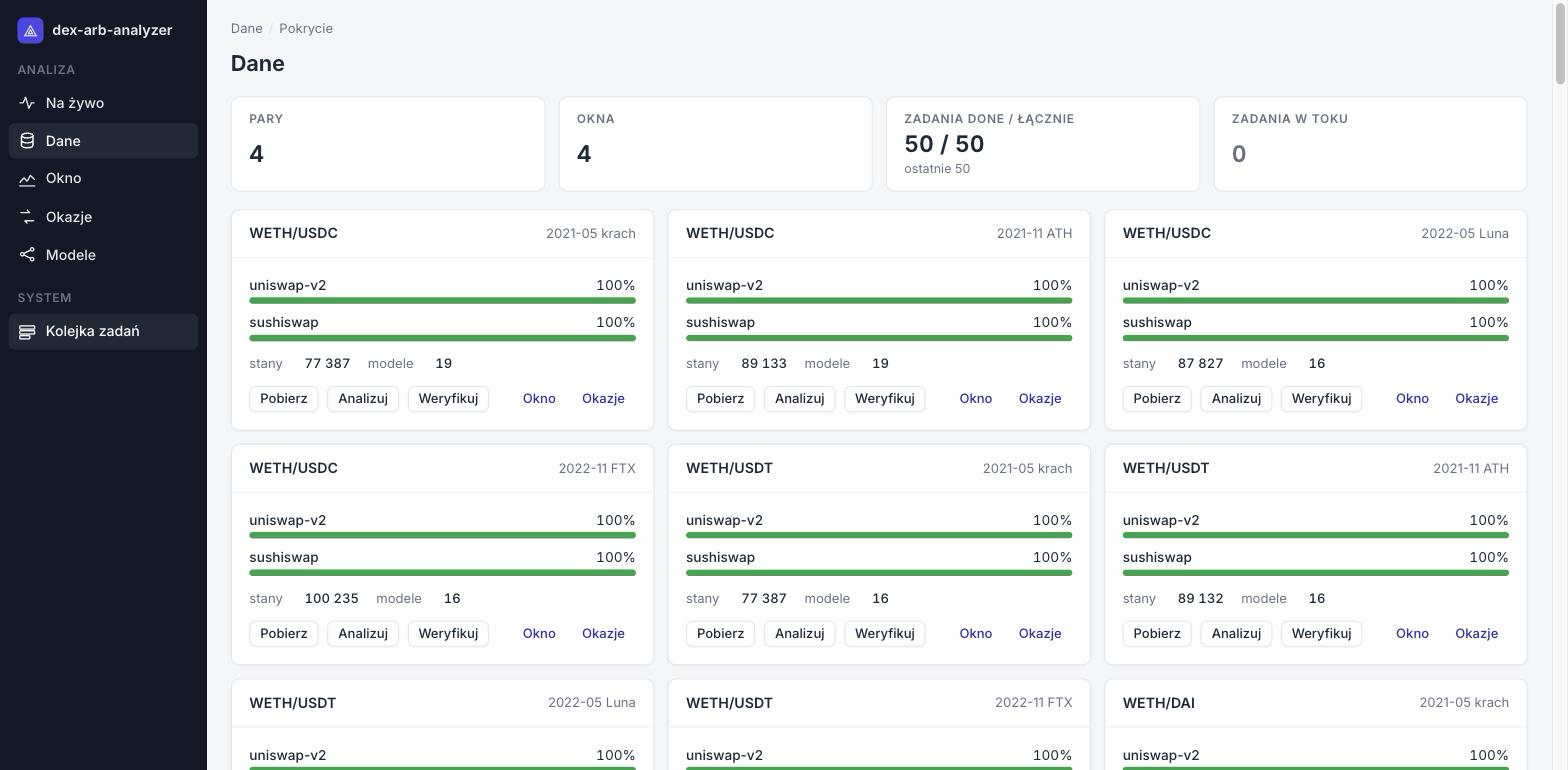
\includegraphics[width=\linewidth]{Images/ui-dane.png}
\caption{Widok \emph{Dane}: pokrycie par i~okien danymi obu pul oraz stan kolejki zadań
(zrzut ekranu, fragment)}\label{fig:ui-dane}
\end{figure}
\begin{figure}[H]\centering
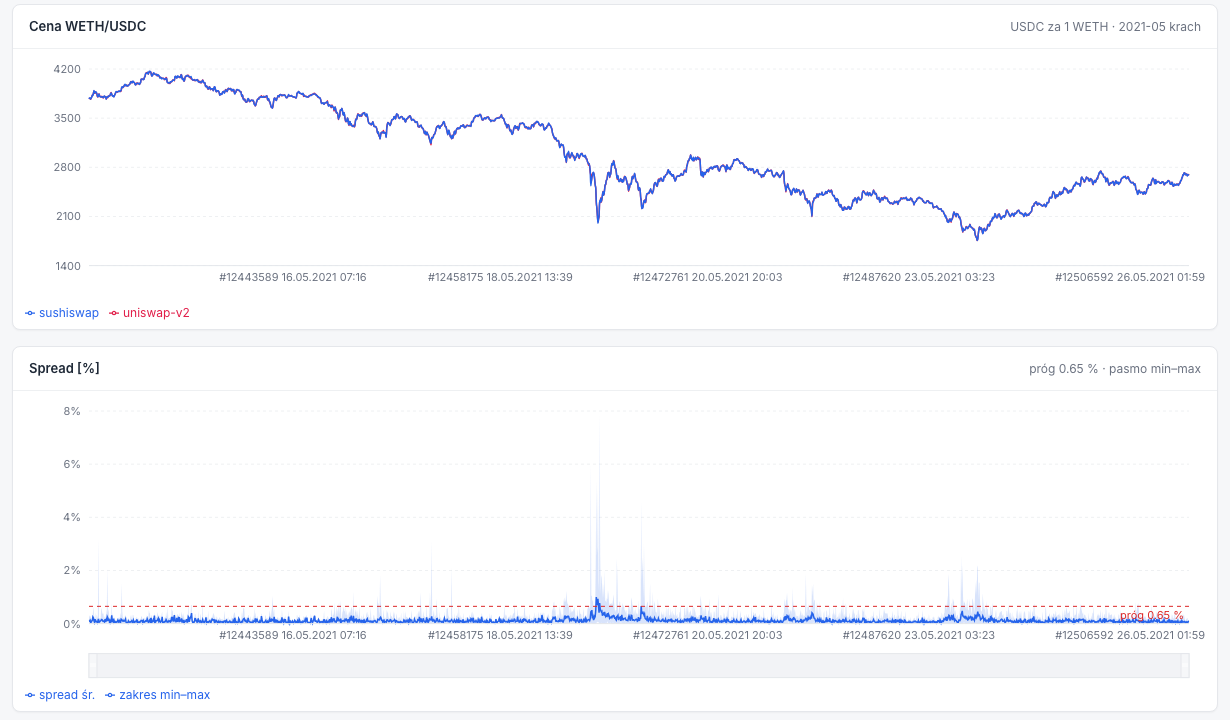
\includegraphics[width=.84\linewidth]{Images/ui-okno.png}
\caption{Widok \emph{Okno}: ceny obu puli i~rozbieżność z~progiem (WETH/USDC, okno 2021-05; zrzut ekranu, fragment)}\label{fig:ui-okno}
\end{figure}
\begin{figure}[H]\centering
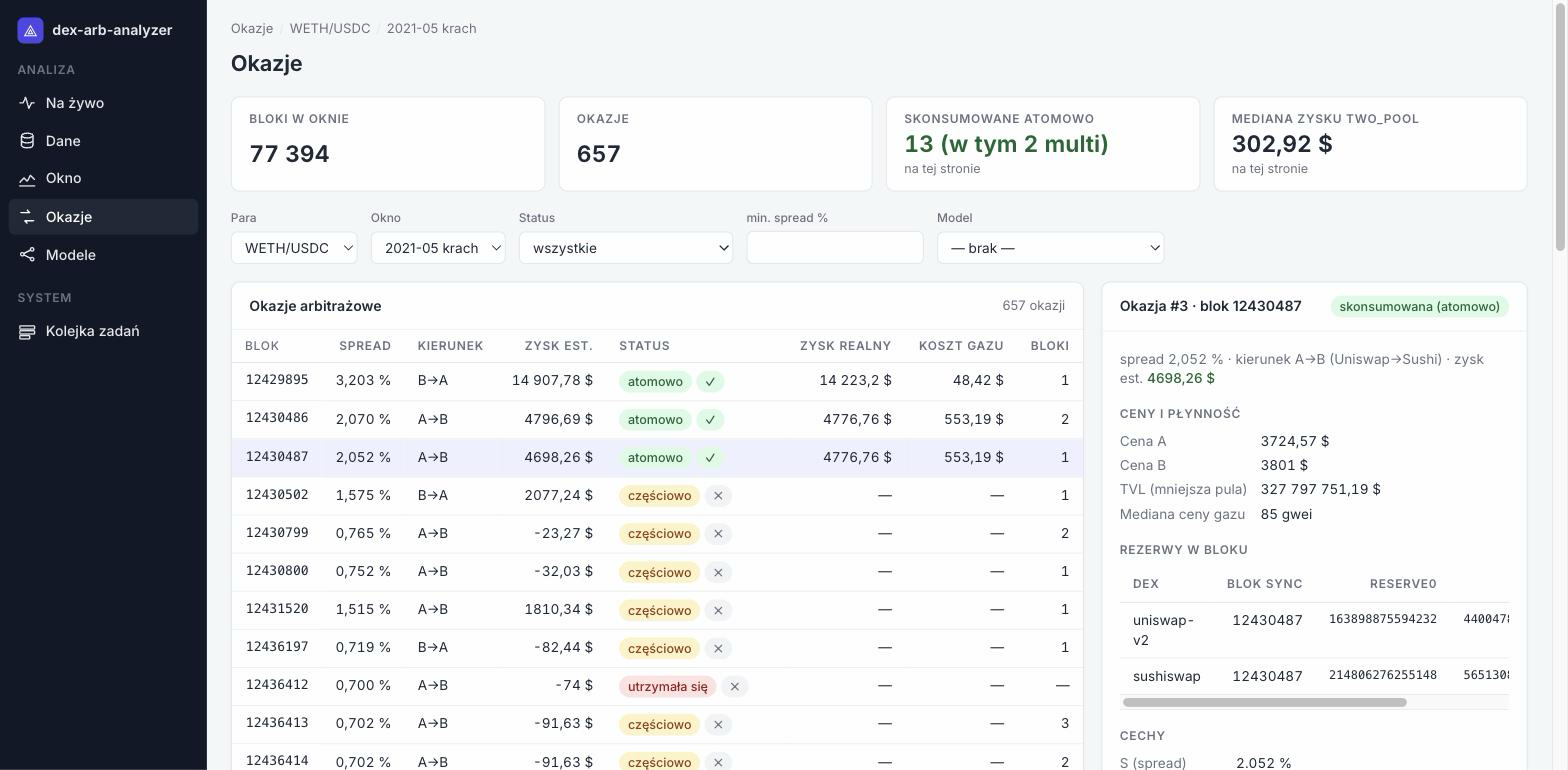
\includegraphics[width=\linewidth]{Images/ui-okazje.png}
\caption{Widok \emph{Okazje}: lista okazji w~oknie z~filtrami, statusem weryfikacji
i~zyskiem zrealizowanym (WETH/USDC, okno 2021-05; zrzut ekranu, fragment)}\label{fig:ui-okazje}
\end{figure}
\begin{figure}[H]\centering
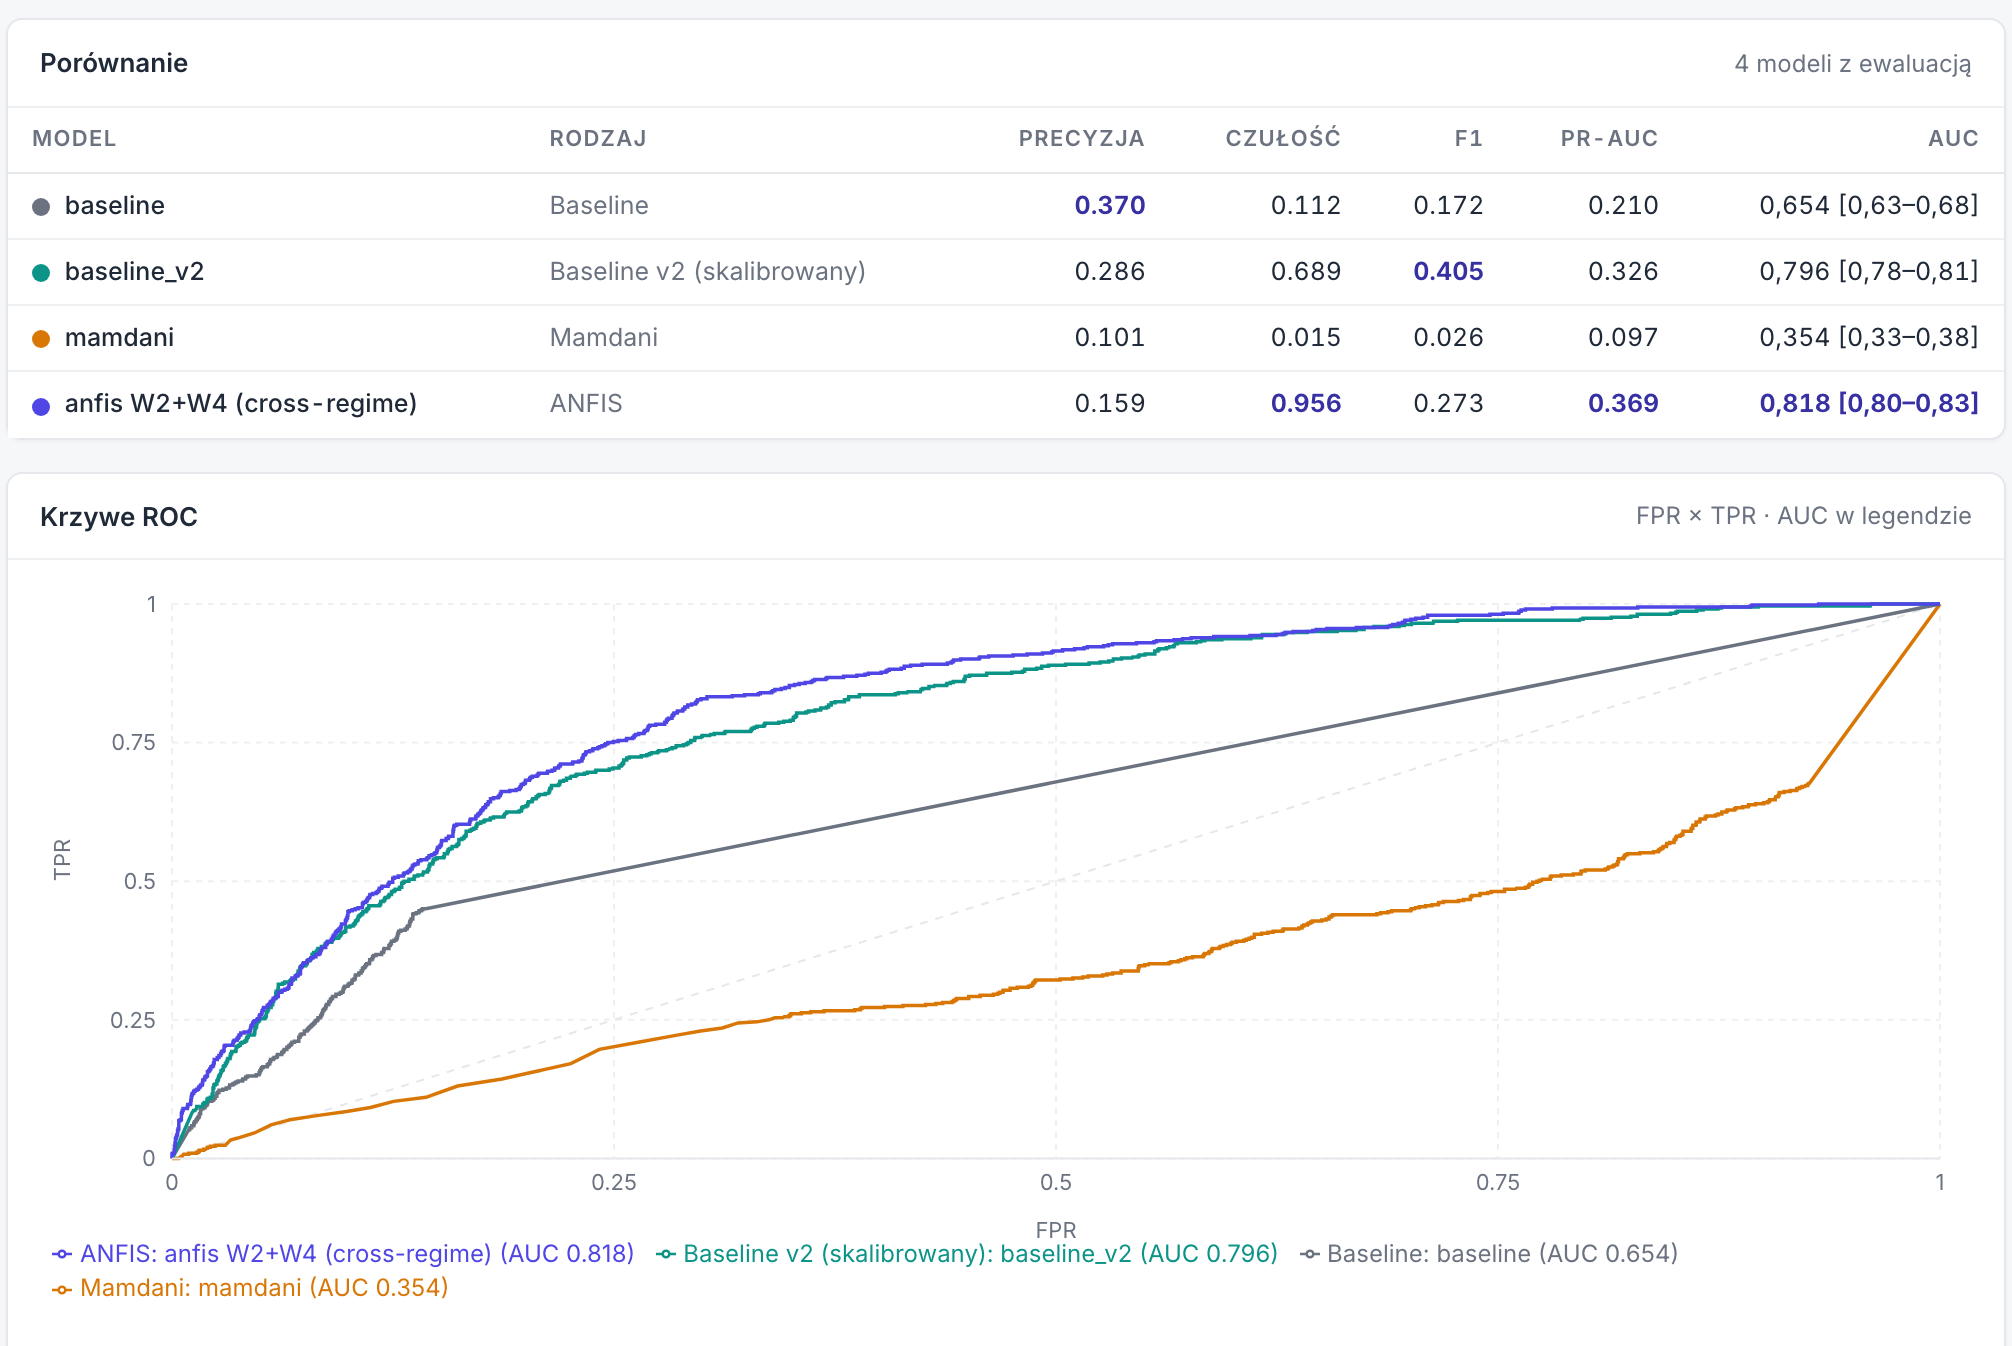
\includegraphics[width=\linewidth]{Images/ui-modele.png}
\caption{Widok \emph{Modele}: tabela metryk i~krzywe ROC czterech modeli na wszystkich oknach (zrzut ekranu, fragment)}\label{fig:ui-modele}
\end{figure}
\begin{figure}[H]\centering
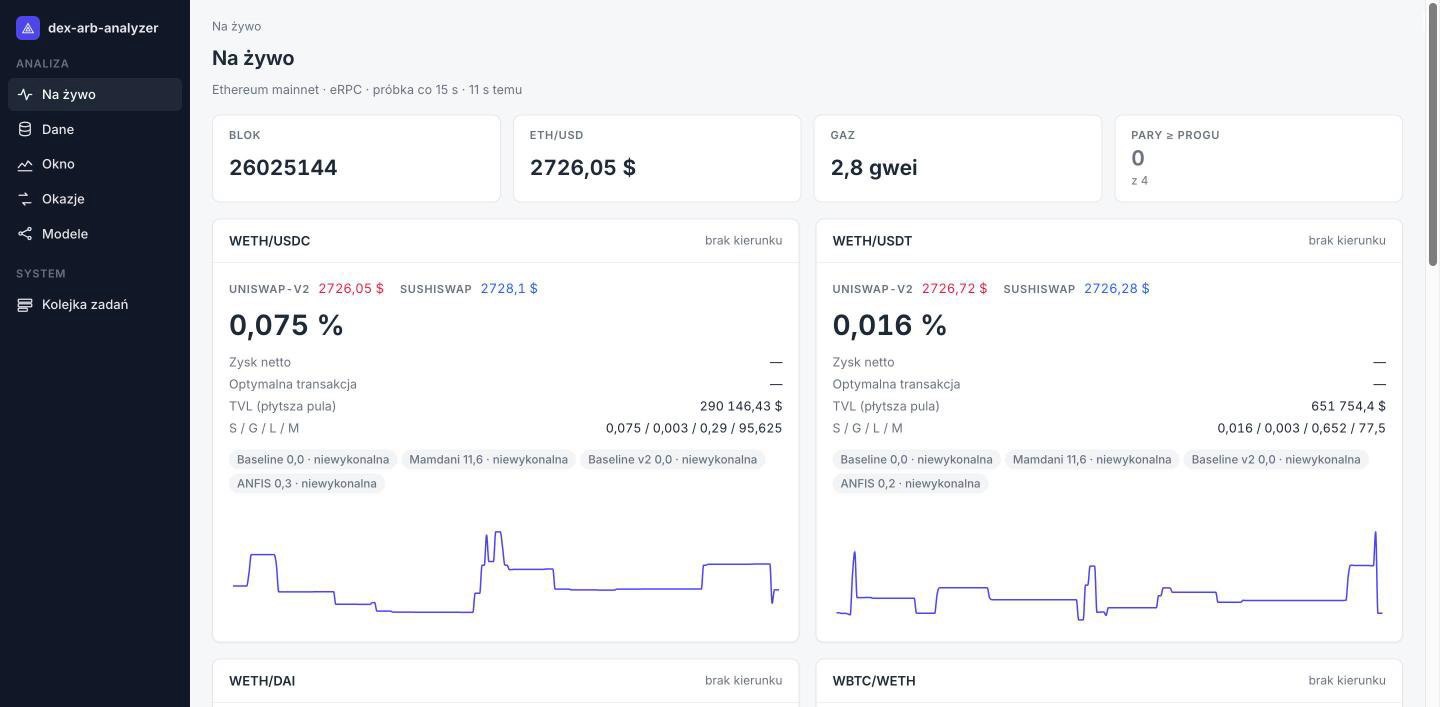
\includegraphics[width=\linewidth]{Images/ui-live.png}
\caption{Widok \emph{Na żywo}: bieżąca rozbieżność cen obu puli, cechy $S/G/L/M$ i~oceny
czterech modeli dla par próbkowanych co 15~s (zrzut ekranu, fragment)}\label{fig:ui-live}
\end{figure}
